\section{Ray-tracing}
While the radatiave transfer equation can be used to solve for brightness temperatures from an orbiting spacecraft, the formalism only holds true for an infinitely narrow beamwidth. The formalism also neglects the effects of refraction between atmospheric layers. Here we present the ray tracing approach used in the developed RTM \cite{Hoffman-thesis}
\subsection{Ray-tracing Described}
Most radio observations of planets are done by measuring emitted rays originating deep in the atmosphere. However for modeling purposes it is easier to model ray-paths originating from the spacecraft and entering in the planet's atmosphere. These are equivalent by reciprocity.

The initial origin of the ray is in the location of the radiometer (either on the spacecraft or on earth) in a cartesian space with the origin defined as the center of the planet. Refer to figure \ref{fig:ray-tracing} for the following discussion. The initial ray direction is set as the pointing direction of the antenna. First the boresight ray-path is calculated. If this does not intersect the outer most atmosphere of the planet the antenna is not pointed toward the planet. Once the ray intersects the first layer, the vector location of this intersection is recorded. From this, the local normal (ray pointing from the origin to the location of intersection) and the zenith angle, can be calculated. The incidence angle is found and Snell's law is applied to find the vector direction of the transmitted ray. Once the vector direction is determined the vector origin of the ray-segment is set as the initial intersection. A new sphere is defined by the next layer and the ray-sphere intersection algorithm is applied with the new inputs. The algorithm calculated the distance and this is recorded. Using the distance the we calculate the new intersection which can be either at the next deeper layer or the previous layer. The latter occurs only when observing from the limb of the planet. This continues until the ray hits the planet, exits from the back of the planet, or becomes so opaque that no significant transmission occurs. 

When the ray hits the planet the incidence angle is recorded and is used to find the emissivity of the planet (Equation \ref{eq:rtm-esurf}, \ref{eq:rtm-rsurf}). If the ray does not hit the surface of the planet the incidence angle is not recorded and no surface temperature is calculated. The ray has a possibility of orbiting the planet, this occurs if the next layer causes critical refraction. When this occurs the layers pathlength gets set to infinity which sets the brightness temperature of the layer to the thermal temperature. The emission from this layer is then attenuated by the layers above.

\begin{figure}[p]
    \centering
	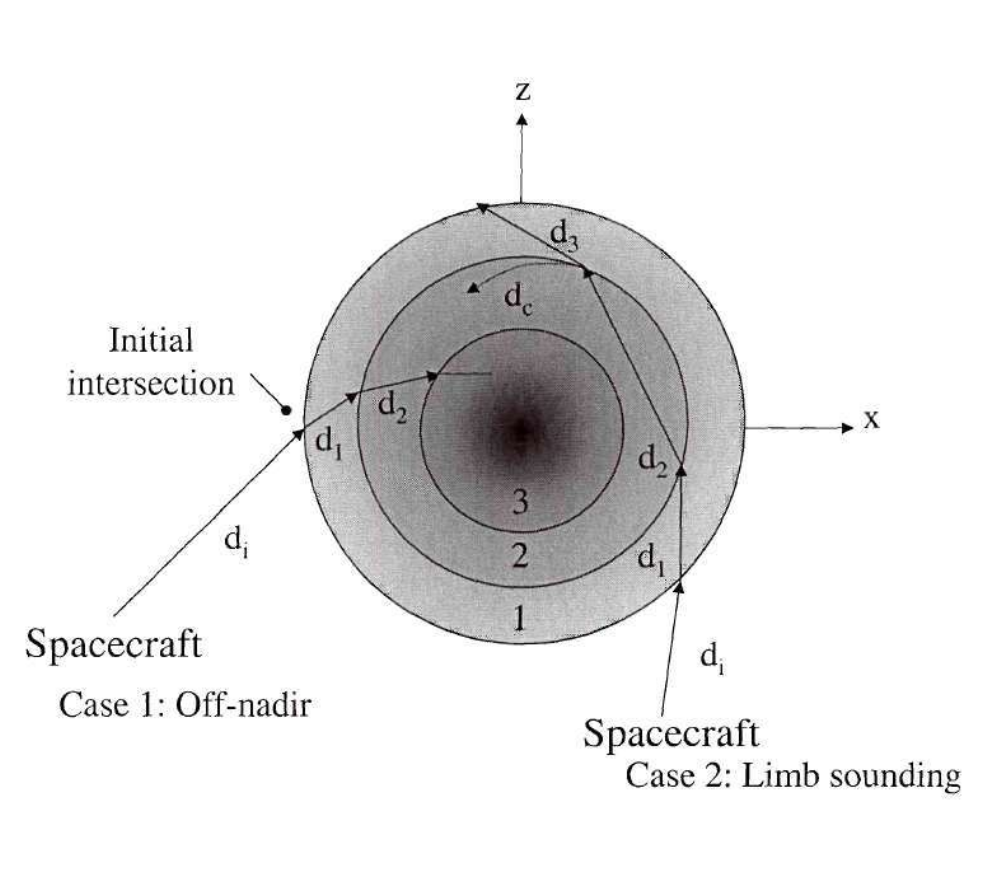
\includegraphics[width=0.7\textwidth]{./rtm/ray-trace.png}
	\caption{A two dimensional graphic example of the ray-tracing process taken from Hoffman 2001 \cite{Hoffman-thesis}. An off-nadir (left) and a limb sounding case (right) are shown. Two possible outcomes for the limb-sounding case are shown. $d_3$ shows the ray exiting the atmosphere, while $d_c$ shows critical refraction.}
		\label{fig:ray-tracing}
\end{figure}

\clearpage
\subsection{Ray-tracing Algorithm Mathematics}
The mathematical foundation for the ray-tracing component of the RTM is developed in this section. The ray-sphere intersection algorithm begins with definition of the parametric equation for a ray. A ray is defined as,
\begin{equation}
\begin{split}
R_{origin} = R_o = \left[ \begin{matrix} X_o&Y_o&Z_o \end{matrix}\right]\\
R_{direction} = R_d = \left[ \begin{matrix} X_d&Y_d&Z_d \end{matrix}\right]
\end{split}
\end{equation}
where
\begin{equation}
\|R_d\|_2^2 = 1
\end{equation}
which defines a ray as a set of points described by the equation for a line
\begin{equation}\label{eq:ray-point}
R = R_o + R_d \times t
\end{equation}
where $T>0$. The sphere is defined by,
\begin{equation}
\begin{split}
S_{center} = S_c = \left[ \begin{matrix} X_c&Y_c&Z_c \end{matrix}\right]\\
S_{radius} = S_r \\
S_{surface} = S_s = \left[ \begin{matrix} X_s&Y_s&Z_s \end{matrix}\right]\\
\end{split}
\end{equation}
where
\begin{equation} \label{eq:ray-sphereprop}
\| S_s - S_c \|_2^2 = S_r^2
\end{equation}
Using equation \ref{eq:ray-point} as the intersection equation for the ray we can substitute that into equation \ref{eq:ray-sphereprop}, resulting in,
\begin{equation}
\| (R_o +R_d \times t) - S_c \|_2^2 = S_r^2
\end{equation}
which can be expanded to
\begin{equation}
(X_o +X_dt - X_c)^2 + (Y_o +Y_dt - Y_c)^2 + (Z_o +Z_dt - Z_c)^2 = S_r^2
\end{equation}
This can be simplified into a quadratic equation
\begin{equation}
At^2 + Bt+C =0
\end{equation}
where,
\begin{eqnarray}
A &=& \|R_d\|_2^2 = 1\\
B &=& 2 \left( \left( R_o -S_c \right) \bullet R_d \right)\\
C &=& \| R_o - S_c \|_2^2 - S_r^2
\end{eqnarray}

The solutions to this equation are the standard quadratic solutions
\begin{equation}
t_{0,1} = \frac{-B\pm\sqrt{B^2-4AC}}{2A}
\end{equation}
where the t's (solutions) are the distance to the intersection point from the ray origin. If the discriminant of these equations is negative the ray misses the sphere. For the purpose of the RTM these are the cases where the ray misses the planet or it exits out of the planet's atmosphere. The smallest positive $t$ alue is the correct solution. Once the t is found the vector location of the intersection is
\begin{equation}
r_{int} = r_i = \left[ \begin{matrix} x_i&y_i&z_i \end{matrix}\right] = \left[ \begin{matrix} X_o + X_dt&Y_o + Y_dt&Z_o + Z_dt \end{matrix}\right]\\
\end{equation}
and the unit vector normal at the surface is then
\begin{equation}
r_{normal} = r_n = \frac{(r_i-S_c)}{S_r} =\left[ \begin{matrix} \frac{(x_i-X_c)}{S_r} &\frac{(y_i-Y_c)}{S_r} & \frac{(z_i-Z_c)}{S_r} \end{matrix}\right]
\end{equation}

In terms of the RTM, the solution to the quadratic equation ($t$) is the distance the ray travels through a given layer. The origin of the transmitted ray is set at the intersection location $r_{int}$ and the direction of the transmitted ray is calculated from the intersection $r_{int}$ and the surface normal $r_{normal}$, using Snell's law.

The vector form of Snell's law needs two vector, the incident ray vector ($\textbf{I}$) and the local surface normal ($\textbf{N}$). Refer to Figure \ref{fig:incident} for a graphical demonstration. The incident angle is calculated using
\begin{equation}
\cos (\theta_1) = -\textbf{I} \bullet \textbf{N}
\end{equation}
From Snell's law, the relative index of refraction ($\eta$) is,
\begin{equation}
\eta = \frac{\sin (\theta_2)}{\sin(\theta_1)} = \frac{\eta_1}{\eta_2}
\end{equation}
The angle of the transmitted ray ($\theta_2$) can be computed from known quantities,
\begin{equation}
\cos(\theta_2) = \sqrt{\left(1-\sin^2(\theta_2\right)}= \sqrt{\left(1-\eta^2\sin^2(\theta_1)\right)} =  \sqrt{\left(1-\eta^2(1-\cos^2(\theta_1))\right)}
\end{equation}
The vector direction of the transmitted ray is computed as,
\begin{equation}
\textbf{T} = \eta\textbf{I} + (\eta\cos(\theta_1) -\cos (\theta_2))\textbf{N}
\end{equation}
the values of \textbf{I} and \textbf{N} are the vectors $R_d$ and $r_n$ respectively. The output of this formula (\textbf{T}) is the new value for $R_d$. Using this algorithm and techniques described in the previous sections we can trace a path through each layer of the atmosphere.

\begin{figure}[!p]
    \centering
	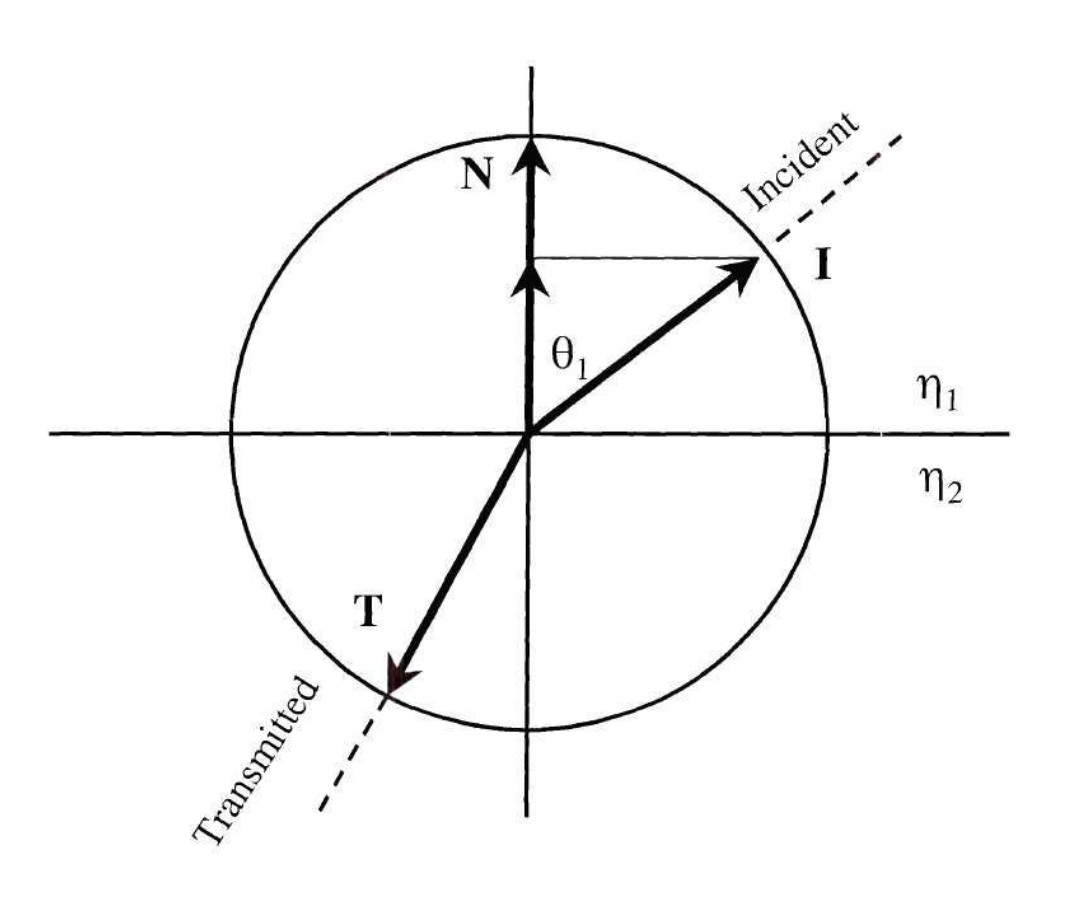
\includegraphics[width=0.7\textwidth]{./rtm/incident.png}
	\caption{Vector implementation of Snell's Law. Image courtesy of Hoffman 2001 \cite{Hoffman-thesis}}
		\label{fig:incident}
\end{figure}
\clearpage
